% ==============================================================================
% PLANTILLA DE INFORME - PFM02 / IIIEPE / MAEM
% ==============================================================================
% Uso:
% 1. Duplica este archivo y renombra la copia por unidad, sesion y actividad.
% 2. Actualiza documenttitle, documentsubtitle, documentsubject, sesionname,
%    activityname, docente y fecha de entrega.
% 3. Lee la consigna del EVA/posgrado y NO pegues las instrucciones completas
%    dentro del producto final. Usa la consigna como lista de cumplimiento.
% 4. Revisa la bibliografia indicada, toma notas, registra citas y redacta con
%    comprension propia.
% 5. Identifica el producto academico o didactico solicitado y construyelo dentro
%    del documento siempre que sea posible.
% 6. Entrega en PDF con la nomenclatura indicada por la unidad de aprendizaje.
%
% Formato institucional recomendado para IIIEPE:
% - Fuente tipo Helvetica, equivalente visual a Arial.
% - Interlineado 1.5.
% - Citas autor-anio con natbib: usar \citep{clave} o \citet{clave}.
% - Referencias en bibliografia BibTeX, formato APA 7 en cuerpo y referencias.
% - Caratula, resumen breve, desarrollo, producto solicitado, conclusion y
%   bibliografia.
% - Redaccion academica clara, coherente, cohesionada, formal y sin faltas.
% - Portada con identidad IIIEPE, programa MAEM, matricula y correo institucional.
% - La portada puede llevar una marca de agua institucional discreta; ajustar
%   las variables coverwatermark... si se requiere apagarla o cambiar intensidad.
%
% Criterios generales de cumplimiento:
% - Responder exactamente a la actividad solicitada en el EVA o por la figura docente.
% - Alinear contenido matematico, PDA, aprendizaje de la secuencia, fases,
%   evaluacion y retroalimentacion.
% - Identificar conceptos, elementos, criterios o categorias de forma precisa.
% - Analizar, interpretar y tomar postura; no solo copiar fuentes.
% - Organizar la informacion por jerarquia, secuencia y criterios claros.
% - Incluir conclusion personal cuando la actividad lo permita o lo solicite.
% - Usar citas y referencias en APA 7.
% - Evitar copiar las indicaciones de la actividad en el cuerpo final.
%
% Regla para productos visuales:
% - Si la actividad pide tabla, cuadro comparativo, esquema, mapa conceptual,
%   mapa mental, linea de tiempo, diagrama, matriz, lista de verificacion, red
%   conceptual, SQA, organizador grafico o producto similar, realizarlo
%   preferentemente con LaTeX/TikZ para mantener nitidez, evidencia editable y
%   diseno controlado.
% - Si la consigna exige Canva, Miro u otra herramienta externa, insertar una
%   captura nitida y conservar la explicacion dentro del documento.
% - Para tablas extensas, usar pagina limpia, sin encabezados ni pies, landscape,
%   letra pequena y restaurar el estilo al terminar.
%
% Criterios de redaccion personal:
% - No escribir para llenar espacio; escribir para sostener una idea.
% - Convertir informacion en criterio: que significa, como funciona, que problema
%   resuelve, que limite presenta y que consecuencia produce.
% - Estructura mental recomendada: problema -> sistema -> consecuencia -> postura.
% - Usar pensamiento de diagnostico: entrada -> proceso -> salida.
% - Cada parrafo debe tener funcion: presentar, explicar, comparar, valorar o
%   concluir.
% - Usar primera persona con moderacion academica: "Considero que",
%   "Desde esta perspectiva", "La posicion que sostengo es". Evitar "yo creo".
%
% Notas de enfoque personal segun enfoque_personal.txt:
% - La voz debe ser academica, tecnica, directa, estrategica y funcional.
% - El texto no debe sonar como estudiante pasivo que recopila: debe sonar como
%   alguien que interpreta, ordena, cruza datos y busca consecuencia practica.
% - Antes de redactar, identificar la funcion de cada seccion: abrir problema,
%   definir criterio, demostrar con evidencia, comparar, valorar o concluir.
% - Evitar frases genericas como "es importante porque si" o "desde siempre".
%   Sustituirlas por relaciones verificables: causa, efecto, limite, costo,
%   funcion, riesgo, implicacion o mejora.
% - Cada concepto debe pasar de definicion a analisis. Formula util:
%   concepto -> funcion -> riesgo si se aplica mal -> consecuencia -> postura.
% - La postura personal no debe ser opinion suelta. Debe tener tres piezas:
%   posicion, razon y efecto. Ejemplo: "Considero que X, porque Y; por ello Z".
% - Integrar experiencia o criterio propio sin perder formalidad: no narrar la
%   vida personal, sino usar mirada practica para explicar por que el tema
%   importa en educacion, derecho, instituciones, comunicacion o profesion.
%
% Estilo observado en actividades ya realizadas:
% - Abrir con una tesis concreta:
%   "La ensenanza de las matematicas no solo transmite procedimientos:
%   organiza formas de razonar, representar y justificar."
% - Formular el problema en negativo y positivo:
%   "El problema no es solo..., sino..."
% - Convertir el producto visual en argumento:
%   "El cuadro no solo recopila datos; reconstruye la funcion, el problema y el
%   punto que requiere correccion."
% - Cerrar con aprendizaje transferible:
%   "No basta con saber que dice la norma; tambien debe analizarse a quien
%   protege, a quien excluye y que razones permiten defenderla publicamente."
%
% Nivel cognitivo esperado:
% - Recordar: usar solo para definir conceptos basicos. No debe ser el nivel
%   dominante en una actividad ponderable.
% - Comprender: explicar con palabras propias y relacionar con el tema.
% - Aplicar: llevar el concepto a un caso, norma, texto, correo, dilema o hecho.
% - Analizar: separar elementos, detectar causas, efectos, tensiones y limites.
% - Evaluar: sostener una postura con criterios, fuentes y consecuencias.
% - Crear: elaborar producto propio: mapa, cuadro, linea de tiempo, ensayo,
%   propuesta, reformulacion, glosario, portafolio o solucion argumentada.
%
% Regla de nivel minimo:
% - Si la actividad vale puntos y pide producto, no quedarse en recordar o
%   comprender. Debe llegar por lo menos a aplicar y analizar; si pide conclusion
%   o postura, debe llegar a evaluar.
%
% Uso de tecnicas didacticas:
% - Esta plantilla conserva el manual "Tecnicas didacticas del aprendizaje" como
%   apoyo para construir productos visuales, analiticos y reflexivos.
% - Cuando la actividad mencione una tecnica didactica, identificar: definicion
%   de la tecnica, producto esperado, pasos de construccion, criterios de revision
%   y cierre reflexivo.
% - La tecnica didactica no debe verse como adorno. Debe mostrar seleccion,
%   jerarquia, relacion entre ideas y lectura propia.
% - Siempre que sea viable, construir la tecnica en LaTeX/TikZ: cuadro
%   comparativo, mapa conceptual, esquema, mapa mental, linea de tiempo, matriz,
%   red conceptual, diagrama de flujo, tabla SQA o lista de verificacion.
%
% Checklist antes de entregar:
% [ ] El titulo, unidad de aprendizaje, sesion, docente y fecha estan actualizados.
% [ ] El objetivo coincide con la consigna del EVA/posgrado.
% [ ] El contenido, PDA y aprendizaje de la secuencia estan alineados.
% [ ] La actividad considera las cinco fases de PFM02 cuando se trate de una secuencia.
% [ ] La practica incluye mecanizacion, variacion y al menos una situacion en contexto.
% [ ] La evaluacion mide el aprendizaje declarado y no solo la repeticion del algoritmo.
% [ ] El producto solicitado aparece visible, rotulado y completo.
% [ ] La introduccion plantea un problema o postura, no solo anuncia el tema.
% [ ] El desarrollo explica, conecta y analiza.
% [ ] Hay citas APA autor-anio dentro del texto.
% [ ] La bibliografia final coincide con las fuentes citadas.
% [ ] La conclusion responde que se comprendio y que postura se sostiene.
% [ ] El nivel cognitivo llega al menos a aplicacion y analisis.
% [ ] Si hay conclusion/postura, incluye posicion, razon y consecuencia.
% [ ] La tecnica didactica solicitada esta construida y explicada.
% [ ] No aparecen instrucciones copiadas de la consigna dentro del producto.
% [ ] Ortografia, acentos, sintaxis y nombres propios revisados.
% [ ] Si se uso IA como apoyo, el texto fue comprendido, revisado y apropiado.
% ==============================================================================

% CREACION DEL DOCUMENTO
\documentclass[
	spanish,
	letterpaper, oneside
]{article}

% ==============================================================================
% INFORMACION DEL DOCUMENTO
% Actualizar en cada actividad.
% Ejemplos:
% \def\documenttitle {Suma y resta con fracciones}
% \def\documentsubtitle {Actividad X - Nombre de la asignatura}
% \def\documentsubject {Sesion 02 -- Secuencia didactica con solucion de actividades}
% ==============================================================================
\def\documenttitle {Suma y resta con fracciones}
\def\documentsubtitle {PFM02 - Temas selectos de matematicas I}
\def\documentsubject {Sesion 02 -- Secuencia didactica con solucion de actividades}

\def\documentauthor {Mtro. Martin Jonathan de la Cruz Munoz}
\def\coursename {Temas selectos de matematicas I}
\def\coursecode {PFM02}

\def\universityname {Instituto de Investigacion, Innovacion y Estudios de Posgrado para la Educacion \\ del Estado de Nuevo Leon}
\def\universityfaculty {Maestria en Aprendizaje y Ensenanza de las Matematicas}
\def\universitydepartment {Temas selectos de matematicas I}
\def\universitydepartmentimage {img/iiiepe/marca-iiiepe.png}
\def\universitydepartmentimagecfg {height=1.75cm}
\def\universitylocation {Monterrey, Nuevo Leon}

% DATOS FIJOS DEL POSGRADO
\def\studentfullname {Mtro. Martin Jonathan de la Cruz Munoz}
\def\studentid {00841}
\def\studentemail {martin.delacruz@campus.iiiepe.edu.mx}
\def\institutionurl {https://iiiepe.edu.mx/}
\def\programperiod {1er tetramestre marzo--julio 2026}
\def\programmodality {Modalidad presencial}
\def\programshort {MAEM}
\def\maemsource {https://iiiepe.edu.mx/maestria-en-aprendizaje-y-ensenanza-de-las-matematicas/}
\def\coursegroup {Grupo A}
\def\courseperiod {Marzo--julio 2026}
\def\evaname {EVA posgrado}
\def\activityname {S02 -- Suma y resta con fracciones}
\def\sessionname {Sesion 02}
\def\blockname {Bloque 1: Numeros racionales y operaciones}
\def\methodology {Aprendizaje basado en indagacion}
\def\steamenfoque {STEAM como enfoque}
\def\curriculumsource {Programa Sintetico Fase 6}
\def\formativefield {Saberes y Pensamiento Cientifico}
\def\mainproduct {Informe academico con secuencia didactica matematica}
\def\docentename {Mtro. Jonathan Cardenas (Coordinador PFM02)}

% INTEGRANTES, PROFESORES Y FECHAS
\def\authortable {
	\begin{tabular}{ll}
		\textbf{Alumno:}
		& \begin{tabular}[t]{l}
			 \studentfullname \\
		\end{tabular} \\
		Matricula: & \studentid \\
		Correo institucional: & \studentemail \\

		\textit{Figura docente:}
		& \begin{tabular}[t]{l}
			\docentename
		\end{tabular} \\
		Unidad: & \coursename \\
		Clave: & \coursecode \\
		Grupo: & \coursegroup \\
		Sesion/Bloque: & \sessionname\ / \blockname \\
		Actividad: & \activityname \\
		Programa: & \programshort \\
		Periodo: & \courseperiod \\
		& \\
		\multicolumn{2}{l}{Fecha de realizacion: \today} \\
		\multicolumn{2}{l}{\universitylocation}
	\end{tabular}
}

% IMPORTACION DEL TEMPLATE BASE
\input{template}

% FORMATO GENERAL
\usepackage{helvet}
\renewcommand{\familydefault}{\sfdefault}

% IDENTIDAD VISUAL IIIEPE
\definecolor{iiiepeNavy}{HTML}{163B5C}
\definecolor{iiiepeBlue}{HTML}{1F6F9F}
\definecolor{iiiepeAqua}{HTML}{20B7A8}
\definecolor{iiiepeOrange}{HTML}{F28C28}
\definecolor{iiiepePaper}{HTML}{F6F8F7}
\definecolor{iiiepeInk}{HTML}{1E2A32}
\definecolor{iiiepeMuted}{HTML}{667085}
\def\portraittitlecolor {iiiepeNavy}

% TABLAS Y PRODUCTOS VISUALES
\usepackage{array}
\usepackage{tabularx}
\usepackage{makecell}
\usepackage{longtable}
\usepackage{etoolbox}
\usepackage{pdflscape}
\usepackage{tikz}
\setlength{\LTcapwidth}{\textwidth}
\makeatletter
\newcommand{\PFMTableSetup}{%
	\ifdim\f@size pt>9.1pt\small\fi
	\renewcommand{\arraystretch}{1.35}%
	\setlength{\tabcolsep}{4pt}%
	\rowcolors{2}{gray!10}{white}%
}
\AtBeginEnvironment{longtable}{\PFMTableSetup}
\AtEndEnvironment{longtable}{\rowcolors{2}{}{}}
\makeatother
\usetikzlibrary{
	arrows.meta,
	positioning,
	calc,
	matrix,
	fit,
	shapes.geometric,
	decorations.pathreplacing,
	shadows.blur
}

\newcommand{\DividirEntre}[2]{\ensuremath{#1\,\text{ entre }\,#2}}

\tikzset{
	cajaProc/.style={
		draw=iiiepeBlue,
		rounded corners=2mm,
		align=center,
		inner sep=5pt,
		minimum height=8mm,
		font=\small
	},
	cajaDato/.style={
		cajaProc,
		fill=iiiepeBlue!8
	},
	cajaOp/.style={
		cajaProc,
		fill=iiiepeOrange!12
	},
	cajaRes/.style={
		cajaProc,
		fill=iiiepeAqua!12
	},
	flechaProc/.style={
		-{Latex[length=2.5mm]},
		thick,
		draw=iiiepeBlue
	},
	notaProc/.style={
		draw=iiiepeOrange,
		rounded corners=2mm,
		fill=iiiepeOrange!12,
		align=center,
		inner sep=4pt,
		font=\scriptsize
	},
	decisionProc/.style={
		diamond,
		aspect=2.1,
		draw=iiiepeBlue,
		fill=iiiepeAqua!10,
		align=center,
		inner sep=2pt,
		font=\scriptsize
	}
}

\newcommand{\RutaOperacion}[4]{%
\begin{tikzpicture}[node distance=8mm]
	\node[cajaDato] (a) {#1};
	\node[cajaOp, right=of a] (b) {#2};
	\node[cajaOp, right=of b] (c) {#3};
	\node[cajaRes, right=of c] (d) {#4};
	\draw[flechaProc] (a) -- (b);
	\draw[flechaProc] (b) -- (c);
	\draw[flechaProc] (c) -- (d);
\end{tikzpicture}%
}

% CITAS EN FORMATO AUTOR-ANIO, COMPATIBLE CON APA 7 EN EL CUERPO DEL TEXTO
% Usar:
% - Cita parentetica: \citep{clave}
% - Cita narrativa: \citet{clave}
% - Varias fuentes: \citep{clave1,clave2}
\setcitestyle{authoryear,open={(},close={)}}

% ==============================================================================
% AYUDAS DE REDACCION
% Quitar o comentar \pendiente cuando el documento final este terminado.
% ==============================================================================
\newcommand{\pendiente}[1]{\textcolor{red}{[PENDIENTE: #1]}}

% ==============================================================================
% MARCA DE AGUA EN PORTADA
% - Se aplica solo a la portada porque usa \AddToShipoutPictureBG*.
% - Para apagarla en alguna actividad: \def\coverwatermarkenabled {false}
% - Usar opacidad baja para que no compita con titulo, datos ni logotipo.
% ==============================================================================
\def\coverwatermarkenabled {true}
\def\coverwatermarkimage {img/iiiepe/logo-puntos.png}
\def\coverwatermarkopacity {0.09}
\def\coverwatermarkwidth {0.58\paperwidth}
\def\coverwatermarkxshift {0cm}
\def\coverwatermarkyshift {-0.15cm}

\newcommand{\insertcoverwatermark}{%
	\ifthenelse{\equal{\coverwatermarkenabled}{true}}{%
		\AddToShipoutPictureBG*{%
			\begin{tikzpicture}[remember picture,overlay]
				\node[
					opacity=\coverwatermarkopacity,
					inner sep=0pt,
					xshift=\coverwatermarkxshift,
					yshift=\coverwatermarkyshift
				] at (current page.center) {%
					\includegraphics[width=\coverwatermarkwidth]{\coverwatermarkimage}%
				};
			\end{tikzpicture}%
		}%
	}{}%
}

\begin{document}

% PORTADA
\insertcoverwatermark
\templatePortrait

% CONFIGURACION DE PAGINA Y ENCABEZADOS
\templatePagecfg
\onehalfspacing

% ==============================================================================
% RESUMEN / ABSTRACT
% Debe ser breve. Formula recomendada:
% Tema + objetivo + tecnica/producto + enfoque personal.
% ==============================================================================
\begin{abstractd}
	\textbf{Objetivo:} Actualizar la actividad de la Sesion 02 para resolver y explicar procedimientos de suma y resta con fracciones, integrando la estructura institucional de secuencia didactica y los criterios generales de evaluacion del curso.

	\textbf{Contenido:} Extension del significado de las operaciones y sus relaciones inversas.

	\textbf{PDA:} Reconoce el significado de las cuatro operaciones basicas y sus relaciones inversas al resolver problemas que impliquen el uso de numeros con signo.

	\textbf{Aprendizaje de la secuencia:} Resolver situaciones problematicas que involucran sumar o restar fracciones.

	\textbf{Producto:} Reporte academico con procedimientos explicitos, ejercicios resueltos, situaciones contextualizadas, autoevaluacion y retroalimentacion.
\end{abstractd}

% TABLA DE CONTENIDOS - INDICE
\templateIndex

% CONFIGURACIONES FINALES
\templateFinalcfg

% ======================= INICIO DEL DOCUMENTO =======================

% ==============================================================================
% SECCION 1: INTRODUCCION
% Apertura recomendada:
% - Iniciar con una afirmacion clara, no con una frase generica.
% - Traducir la consigna a un problema academico, didactico, matematico,
%   pedagogico o profesional, segun la unidad de aprendizaje.
% - Explicar por que importa.
% - Cerrar anticipando el enfoque personal.
% ==============================================================================
\section{Introduccion}

La suma y la resta con fracciones exigen mas que aplicar una regla mecanica: requieren reconocer que solo se pueden combinar partes comparables cuando estan expresadas con la misma unidad de referencia. Por ello, el denominador comun no se presenta como un tramite algebraico, sino como la estrategia que permite expresar las fracciones en unidades equivalentes antes de operar numeradores.

Esta actividad se organiza conforme a la estructura institucional de la secuencia didactica de PFM02: antecedente del contenido, introduccion y explicacion, practica, evaluacion y retroalimentacion. Tambien toma en cuenta los criterios generales de evaluacion del curso, donde las actividades diarias, la exposicion de secuencias, el escrito reflexivo y la exposicion final deben mostrar claridad conceptual, procedimiento visible, aplicacion contextual y reflexion sobre el aprendizaje.

El enfoque del reporte es pedagogico y operativo: cada procedimiento indica que se hace, por que funciona y como se comprueba el resultado. Asi, la actividad no queda reducida a una lista de respuestas, sino a una secuencia que permite al estudiante anticipar, operar, simplificar, interpretar y verificar.

\section{Desarrollo de la actividad}

\subsection{Datos base de la secuencia}

\begin{longtable}{@{}p{0.28\linewidth}p{0.65\linewidth}@{}}
	\caption{Datos institucionales de la Sesion 02}\label{tab:datos-sesion02}\\
	\toprule
	\textbf{Elemento} & \textbf{Descripcion} \\
	\midrule
	\endfirsthead
	\toprule
	\textbf{Elemento} & \textbf{Descripcion} \\
	\midrule
	\endhead
	Tema & Suma y resta con fracciones. \\
	Contenido & Extension del significado de las operaciones y sus relaciones inversas. \\
	Proceso de desarrollo de aprendizaje & Reconoce el significado de las cuatro operaciones basicas y sus relaciones inversas al resolver problemas que impliquen el uso de numeros con signo. \\
	Aprendizaje de la secuencia & Resolver situaciones problematicas que involucran sumar o restar fracciones. \\
	Producto esperado & Procedimientos escritos, ejercicios resueltos, situaciones en contexto, autoevaluacion y retroalimentacion. \\
	\bottomrule
\end{longtable}

\subsection{Criterios institucionales incorporados}

\begin{longtable}{@{}p{0.26\linewidth}p{0.32\linewidth}p{0.34\linewidth}@{}}
	\caption{Traduccion de criterios institucionales al producto elaborado}\label{tab:criterios-institucionales}\\
	\toprule
	\textbf{Fuente institucional} & \textbf{Criterio recuperado} & \textbf{Aplicacion en este reporte y presentacion} \\
	\midrule
	\endfirsthead
	\toprule
	\textbf{Fuente institucional} & \textbf{Criterio recuperado} & \textbf{Aplicacion en este reporte y presentacion} \\
	\midrule
	\endhead
	Estructura de una secuencia didactica & Cinco fases: antecedente, explicacion, practica, evaluacion y retroalimentacion. & La actividad se organiza como una ruta de aprendizaje: recuperar conocimientos previos, explicar procedimientos, resolver ejercicios, evaluar desempeno y cerrar con metacognicion. \\
	Criterios de evaluacion & Asistencia, actividades diarias, exposicion diaria, escrito reflexivo y exposicion final. & El producto prioriza evidencias observables: procedimiento, respuesta simplificada, interpretacion contextual y reflexion final. \\
	Sesion 02 & Resolver situaciones problematicas que involucran sumar o restar fracciones. & Los ejercicios no solo se contestan; se muestran rutas de solucion y verificacion. \\
	\bottomrule
\end{longtable}

\subsection{Secuencia didactica propuesta}

\begin{longtable}{@{}p{0.12\linewidth}p{0.20\linewidth}p{0.35\linewidth}p{0.25\linewidth}@{}}
	\caption{Organizacion didactica en cinco fases}\label{tab:fases-secuencia}\\
	\toprule
	\textbf{Fase} & \textbf{Funcion} & \textbf{Actividad matematica} & \textbf{Evidencia} \\
	\midrule
	\endfirsthead
	\toprule
	\textbf{Fase} & \textbf{Funcion} & \textbf{Actividad matematica} & \textbf{Evidencia} \\
	\midrule
	\endhead
	1 & Antecedente & Recuperar simplificacion, equivalencia, fracciones propias, impropias y mixtas. & Tabla diagnostica de simplificacion y conversion. \\
	2 & Introduccion y explicacion & Explicar por que se requiere denominador comun para sumar o restar partes. & Apunte con procedimiento y ejemplo guiado. \\
	3 & Practica & Resolver ejercicios de mismo denominador, distinto denominador, producto cruzado y fracciones equivalentes. & Procedimientos completos y resultados simplificados. \\
	4 & Evaluacion & Resolver situaciones en contexto e identificar la operacion necesaria. & Solucion contextual con operacion, desarrollo y respuesta. \\
	5 & Retroalimentacion & Revisar errores frecuentes: no igualar denominadores, olvidar simplificar o confundir suma con resta. & Autoevaluacion y mejora puntual. \\
	\bottomrule
\end{longtable}

\section{Procedimientos matematicos}

\subsection{Idea central: sumar o restar partes comparables}

Para sumar o restar fracciones se debe asegurar que las partes tengan el mismo tamano. Si los denominadores son iguales, las fracciones ya estan expresadas en la misma unidad; por eso se operan los numeradores y se conserva el denominador:
\[
	\frac{a}{c}+\frac{b}{c}=\frac{a+b}{c},
	\qquad
	\frac{a}{c}-\frac{b}{c}=\frac{a-b}{c}.
\]

\begin{figure}[H]
	\centering
	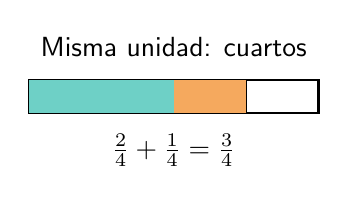
\begin{tikzpicture}[scale=0.92]
		\foreach \i in {0,1,2,3}{\draw[thick] (\i,0) rectangle +(1,0.45);}
		\fill[iiiepeAqua!65] (0,0) rectangle +(1,0.45);
		\fill[iiiepeAqua!65] (1,0) rectangle +(1,0.45);
		\fill[iiiepeOrange!75] (2,0) rectangle +(1,0.45);
		\node[below] at (2,-0.15) {$\frac{2}{4}+\frac{1}{4}=\frac{3}{4}$};
		\node[above] at (2,0.65) {Misma unidad: cuartos};
	\end{tikzpicture}
	\caption{Cuando el denominador es comun, las partes son comparables.}
\end{figure}

\subsection{Fracciones con distinto denominador}

Cuando los denominadores son distintos, primero se construyen fracciones equivalentes con un denominador comun. La opcion pedagogica mas clara es usar el minimo comun multiplo (mcm), porque reduce calculos y facilita la simplificacion:
\[
	\frac{a}{b}+\frac{c}{d}
	=\frac{a\cdot \frac{m}{b}}{m}+\frac{c\cdot \frac{m}{d}}{m}
	=\frac{a\left(\frac{m}{b}\right)+c\left(\frac{m}{d}\right)}{m},
\]
\[
	\text{donde } m=\operatorname{mcm}(b,d).
\]

Ejemplo:
\[
	\frac{3}{4}+\frac{1}{2}=\frac{3}{4}+\frac{2}{4}=\frac{5}{4}=1\,\frac{1}{4}.
\]

\subsection{Producto cruzado como atajo controlado}

El producto cruzado puede usarse para dos fracciones, pero debe explicarse como una forma abreviada de construir un denominador comun, no como una regla aislada:
\[
	\frac{a}{b}+\frac{c}{d}=\frac{ad+bc}{bd},
	\qquad
	\frac{a}{b}-\frac{c}{d}=\frac{ad-bc}{bd}.
\]

Ejemplo de resta:
\[
	\frac{3}{2}-\frac{3}{5}=\frac{3(5)-3(2)}{2(5)}=\frac{15-6}{10}=\frac{9}{10}.
\]

\subsection{Enteros y fracciones mixtas}

Un entero puede escribirse como fraccion con denominador $1$. Una fraccion mixta se transforma en impropia antes de operar:
\[
	n\frac{a}{b}=\frac{nb+a}{b}.
\]

Ejemplo:
\[
	5\,\frac{2}{3}+\frac{2}{8}=\frac{17}{3}+\frac{1}{4}=\frac{68}{12}+\frac{3}{12}=\frac{71}{12}=5\,\frac{11}{12}.
\]

\subsection{Rutas visuales de procedimiento}

Las siguientes rutas sintetizan la accion matematica central de cada procedimiento. Cada flecha indica una transformacion necesaria: identificar la unidad, construir equivalencias, operar y simplificar.

\begin{figure}[H]
	\centering
	\resizebox{0.88\linewidth}{!}{%
		\RutaOperacion
		{$\frac{7}{2}+\frac{5}{2}$}
		{mismos\\medios}
		{$\frac{7+5}{2}$}
		{$\frac{12}{2}=6$}%
	}
	\caption{Ruta visual para operar fracciones con el mismo denominador.}
\end{figure}

\begin{figure}[H]
	\centering
	\resizebox{0.88\linewidth}{!}{%
		\RutaOperacion
		{$\frac{3}{4}+\frac{1}{2}$}
		{mcm $=4$\\unidad comun}
		{$\frac{3}{4}+\frac{2}{4}$}
		{$\frac{5}{4}=1\,\frac{1}{4}$}%
	}
	\caption{Ruta visual para construir denominador comun mediante equivalencias.}
\end{figure}

\begin{figure}[H]
	\centering
	\resizebox{0.88\linewidth}{!}{%
		\RutaOperacion
		{$\frac{1}{2}+\frac{3}{7}$}
		{producto\\de denominadores}
		{$\frac{1(7)+3(2)}{14}$}
		{$\frac{13}{14}$}%
	}
	\caption{Ruta visual del producto cruzado como atajo para denominador comun.}
\end{figure}

\begin{figure}[H]
	\centering
	\resizebox{0.88\linewidth}{!}{%
		\RutaOperacion
		{$5\,\frac{2}{3}$}
		{convertir\\mixta}
		{$\frac{5(3)+2}{3}$}
		{$\frac{17}{3}$}%
	}
	\caption{Ruta visual para convertir una fraccion mixta en impropia antes de operar.}
\end{figure}

\section{Ejercicios de practica resueltos}

\subsection{Simplificacion de fracciones}

La tabla presenta varios incisos resueltos; el esquema posterior muestra la ruta comun que se aplica al bloque completo.

\begin{longtable}{@{}p{0.22\linewidth}p{0.24\linewidth}p{0.22\linewidth}p{0.24\linewidth}@{}}
	\caption{Fracciones simplificadas hasta forma irreductible}\label{tab:simplificacion}\\
	\toprule
	\textbf{Fraccion} & \textbf{Simplificacion} & \textbf{Fraccion} & \textbf{Simplificacion} \\
	\midrule
	\endfirsthead
	\toprule
	\textbf{Fraccion} & \textbf{Simplificacion} & \textbf{Fraccion} & \textbf{Simplificacion} \\
	\midrule
	\endhead
	$\frac{4}{20}$ & $\frac{4/4}{20/4}=\frac{1}{5}$ & $\frac{9}{27}$ & $\frac{9/9}{27/9}=\frac{1}{3}$ \\
	$\frac{6}{24}$ & $\frac{6/6}{24/6}=\frac{1}{4}$ & $\frac{24}{32}$ & $\frac{24/8}{32/8}=\frac{3}{4}$ \\
	$\frac{12}{30}$ & $\frac{12/6}{30/6}=\frac{2}{5}$ & $\frac{15}{25}$ & $\frac{15/5}{25/5}=\frac{3}{5}$ \\
	\bottomrule
\end{longtable}

\begin{figure}[H]
	\centering
	\resizebox{0.82\linewidth}{!}{%
		\RutaOperacion
		{$\frac{4}{20}$}
		{dividir numerador\\y denominador entre $4$}
		{$\frac{4/4}{20/4}$}
		{$\frac{1}{5}$}%
	}
	\caption{Ruta comun para simplificar una fraccion hasta forma irreductible.}
\end{figure}

\subsection{Conversion entre impropias y mixtas}

La tabla presenta varios incisos resueltos; el esquema posterior muestra la ruta comun que se aplica al bloque completo.

\begin{longtable}{@{}p{0.20\linewidth}p{0.28\linewidth}p{0.20\linewidth}p{0.24\linewidth}@{}}
	\caption{Conversion de fracciones impropias a mixtas}\label{tab:impropias-mixtas}\\
	\toprule
	\textbf{Impropia} & \textbf{Mixta} & \textbf{Impropia} & \textbf{Mixta} \\
	\midrule
	\endfirsthead
	\toprule
	\textbf{Impropia} & \textbf{Mixta} & \textbf{Impropia} & \textbf{Mixta} \\
	\midrule
	\endhead
	$\frac{5}{4}$ & $1\,\frac{1}{4}$ & $\frac{50}{3}$ & $16\,\frac{2}{3}$ \\
	$\frac{8}{3}$ & $2\,\frac{2}{3}$ & $\frac{11}{2}$ & $5\,\frac{1}{2}$ \\
	$\frac{7}{4}$ & $1\,\frac{3}{4}$ & $\frac{4}{3}$ & $1\,\frac{1}{3}$ \\
	\bottomrule
\end{longtable}

\begin{figure}[H]
	\centering
	\resizebox{0.82\linewidth}{!}{%
		\RutaOperacion
		{$\frac{50}{3}$}
		{dividir\\$50=16(3)+2$}
		{$16+\frac{2}{3}$}
		{$16\,\frac{2}{3}$}%
	}
	\caption{Ruta comun para convertir una fraccion impropia en mixta.}
\end{figure}

La tabla presenta varios incisos resueltos; el esquema posterior muestra la ruta comun que se aplica al bloque completo.

\begin{longtable}{@{}p{0.20\linewidth}p{0.28\linewidth}p{0.20\linewidth}p{0.24\linewidth}@{}}
	\caption{Conversion de fracciones mixtas a impropias}\label{tab:mixtas-impropias}\\
	\toprule
	\textbf{Mixta} & \textbf{Impropia} & \textbf{Mixta} & \textbf{Impropia} \\
	\midrule
	\endfirsthead
	\toprule
	\textbf{Mixta} & \textbf{Impropia} & \textbf{Mixta} & \textbf{Impropia} \\
	\midrule
	\endhead
	$5\,\frac{3}{2}$ & $\frac{5(2)+3}{2}=\frac{13}{2}$ & $15\,\frac{1}{3}$ & $\frac{15(3)+1}{3}=\frac{46}{3}$ \\
	$9\,\frac{2}{3}$ & $\frac{9(3)+2}{3}=\frac{29}{3}$ & $7\,\frac{7}{8}$ & $\frac{7(8)+7}{8}=\frac{63}{8}$ \\
	$8\,\frac{3}{4}$ & $\frac{8(4)+3}{4}=\frac{35}{4}$ & $2\,\frac{3}{16}$ & $\frac{2(16)+3}{16}=\frac{35}{16}$ \\
	\bottomrule
\end{longtable}

\begin{figure}[H]
	\centering
	\resizebox{0.82\linewidth}{!}{%
		\RutaOperacion
		{$15\,\frac{1}{3}$}
		{multiplicar entero\\por denominador}
		{$\frac{15(3)+1}{3}$}
		{$\frac{46}{3}$}%
	}
	\caption{Ruta comun para convertir una fraccion mixta en impropia.}
\end{figure}

\subsection{Suma y resta con mismo denominador}

La tabla presenta varios incisos resueltos; el esquema posterior muestra la ruta comun que se aplica al bloque completo.

\begin{longtable}{@{}p{0.48\linewidth}p{0.43\linewidth}@{}}
	\caption{Ejercicios con denominador comun}\label{tab:mismo-denominador}\\
	\toprule
	\textbf{Operacion} & \textbf{Procedimiento y resultado} \\
	\midrule
	\endfirsthead
	\toprule
	\textbf{Operacion} & \textbf{Procedimiento y resultado} \\
	\midrule
	\endhead
	$\frac{7}{2}+\frac{5}{2}$ & $\frac{7+5}{2}=\frac{12}{2}=6$ \\
	$\frac{8}{7}+\frac{1}{7}+\frac{2}{7}$ & $\frac{8+1+2}{7}=\frac{11}{7}=1\,\frac{4}{7}$ \\
	$\frac{17}{4}-\frac{10}{4}$ & $\frac{17-10}{4}=\frac{7}{4}=1\,\frac{3}{4}$ \\
	$\frac{12}{9}-\frac{3}{9}-\frac{4}{9}$ & $\frac{12-3-4}{9}=\frac{5}{9}$ \\
	\bottomrule
\end{longtable}

\begin{figure}[H]
	\centering
	\resizebox{0.86\linewidth}{!}{%
		\RutaOperacion
		{$\frac{8}{7}+\frac{1}{7}+\frac{2}{7}$}
		{mismos\\septimos}
		{$\frac{8+1+2}{7}$}
		{$\frac{11}{7}=1\,\frac{4}{7}$}%
	}
	\caption{Ruta comun para sumar fracciones con el mismo denominador.}
\end{figure}

\subsection{Suma y resta con distinto denominador}

La tabla presenta varios incisos resueltos; el esquema posterior muestra la ruta comun que se aplica al bloque completo.

\begin{longtable}{@{}p{0.48\linewidth}p{0.43\linewidth}@{}}
	\caption{Ejercicios mediante producto cruzado}\label{tab:producto-cruzado}\\
	\toprule
	\textbf{Operacion} & \textbf{Procedimiento y resultado} \\
	\midrule
	\endfirsthead
	\toprule
	\textbf{Operacion} & \textbf{Procedimiento y resultado} \\
	\midrule
	\endhead
	$\frac{1}{2}+\frac{3}{7}$ & $\frac{1(7)+3(2)}{14}=\frac{13}{14}$ \\
	$\frac{6}{9}+\frac{2}{10}$ & $\frac{60+18}{90}=\frac{78}{90}=\frac{13}{15}$ \\
	$\frac{3}{2}-\frac{3}{5}$ & $\frac{15-6}{10}=\frac{9}{10}$ \\
	$\frac{10}{3}-\frac{9}{4}$ & $\frac{40-27}{12}=\frac{13}{12}=1\,\frac{1}{12}$ \\
	\bottomrule
\end{longtable}

\begin{figure}[H]
	\centering
	\resizebox{0.86\linewidth}{!}{%
		\RutaOperacion
		{$\frac{1}{2}+\frac{3}{7}$}
		{producto\\cruzado}
		{$\frac{1(7)+3(2)}{14}$}
		{$\frac{13}{14}$}%
	}
	\caption{Ruta comun para resolver con producto cruzado.}
\end{figure}

La tabla presenta varios incisos resueltos; el esquema posterior muestra la ruta comun que se aplica al bloque completo.

\begin{longtable}{@{}p{0.48\linewidth}p{0.43\linewidth}@{}}
	\caption{Ejercicios mediante fracciones equivalentes}\label{tab:equivalentes}\\
	\toprule
	\textbf{Operacion} & \textbf{Procedimiento y resultado} \\
	\midrule
	\endfirsthead
	\toprule
	\textbf{Operacion} & \textbf{Procedimiento y resultado} \\
	\midrule
	\endhead
	$\frac{3}{4}+\frac{1}{2}$ & $\frac{3}{4}+\frac{2}{4}=\frac{5}{4}=1\,\frac{1}{4}$ \\
	$\frac{7}{4}+\frac{3}{20}$ & $\frac{35}{20}+\frac{3}{20}=\frac{38}{20}=\frac{19}{10}$ \\
	$\frac{2}{3}+\frac{1}{7}$ & $\frac{14}{21}+\frac{3}{21}=\frac{17}{21}$ \\
	$\frac{4}{9}-\frac{1}{3}$ & $\frac{4}{9}-\frac{3}{9}=\frac{1}{9}$ \\
	$\frac{7}{15}-\frac{2}{5}$ & $\frac{7}{15}-\frac{6}{15}=\frac{1}{15}$ \\
	$\frac{5}{3}-\frac{4}{27}$ & $\frac{45}{27}-\frac{4}{27}=\frac{41}{27}=1\,\frac{14}{27}$ \\
	\bottomrule
\end{longtable}

\begin{figure}[H]
	\centering
	\resizebox{0.86\linewidth}{!}{%
		\RutaOperacion
		{$\frac{3}{4}+\frac{1}{2}$}
		{convertir\\$\frac{1}{2}=\frac{2}{4}$}
		{$\frac{3}{4}+\frac{2}{4}$}
		{$\frac{5}{4}=1\,\frac{1}{4}$}%
	}
	\caption{Ruta comun para resolver con fracciones equivalentes.}
\end{figure}

\section{Situaciones en contexto resueltas}

\begin{longtable}{@{}p{0.08\linewidth}p{0.42\linewidth}p{0.40\linewidth}@{}}
	\caption{Solucion de situaciones contextualizadas}\label{tab:situaciones-contexto}\\
	\toprule
	\textbf{Sit.} & \textbf{Operacion planteada} & \textbf{Resultado interpretado} \\
	\midrule
	\endfirsthead
	\toprule
	\textbf{Sit.} & \textbf{Operacion planteada} & \textbf{Resultado interpretado} \\
	\midrule
	\endhead
	01 & Para pasar de $4$ a $12$ porciones se multiplica por $3$: agua $1\,\frac{1}{2}\cdot3=\frac{3}{2}\cdot3=\frac{9}{2}$; piloncillo $\frac14\cdot3=\frac34$. & Necesita $4\,\frac12$ tazas de agua y $\frac34$ de taza de piloncillo rallado. \\
	02 & $\frac13+\frac14=\frac{4}{12}+\frac{3}{12}=\frac{7}{12}$. & Luisa y Wendy comieron $\frac{7}{12}$ de pizza. \\
	03 & $1-\bigl(\frac14+\frac12\bigr)=1-\bigl(\frac14+\frac24\bigr)=1-\frac34=\frac14$. & Quedo $\frac14$ de la bolsa. \\
	04 & $\frac{2}{8}+5\,\frac23=\frac14+\frac{17}{3}=\frac{3}{12}+\frac{68}{12}=\frac{71}{12}$. & Karina recorrio $5\,\frac{11}{12}$ km. \\
	05 & $1\,\frac12-\frac64=\frac32-\frac32=0$. & No quedo yeso en la bolsa. \\
	06 & $1-\bigl(\frac18+\frac14\bigr)=1-\bigl(\frac18+\frac28\bigr)=1-\frac38=\frac58$. & El trigo ocupa $\frac58$ del rancho. \\
	07 & $1-\bigl(\frac14+\frac16+\frac13\bigr)=1-\bigl(\frac{3+2+4}{12}\bigr)=\frac{3}{12}=\frac14$. & Sin deporte favorito: $\frac14$ del total. \\
	08 & $4\,\frac12+3\,\frac58+3\,\frac34=\frac{36}{8}+\frac{29}{8}+\frac{30}{8}=\frac{95}{8}$. & Antonio recorrio $11\,\frac78$ km. \\
	09 & $\frac{7}{12}+\frac56+\frac23=\frac{7}{12}+\frac{10}{12}+\frac{8}{12}=\frac{25}{12}$. & Las tablas apiladas miden $2\,\frac{1}{12}$ pulgadas. \\
	10 & Rectangulo de $4\,\frac34$ cm por $2\,\frac12$ cm: $P=2\biggl(\frac{19}{4}+\frac{5}{2}\biggr)=2\biggl(\frac{29}{4}\biggr)=\frac{29}{2}$. & Perimetro: $\frac{29}{2}$ cm; opcion a. \\
	\bottomrule
\end{longtable}

\subsection{Esquemas de apoyo para las situaciones}

Los siguientes esquemas no sustituyen las soluciones de la tabla; muestran la estrategia comun usada para interpretar las situaciones.

\begin{figure}[H]
	\centering
	\resizebox{0.86\linewidth}{!}{%
		\RutaOperacion
		{$\frac{1}{3}+\frac{1}{4}$}
		{denominador\\$12$}
		{$\frac{4}{12}+\frac{3}{12}$}
		{$\frac{7}{12}$}%
	}
	\caption{Esquema de combinacion de cantidades: situacion 02 de la pizza.}
\end{figure}

\begin{figure}[H]
	\centering
	\resizebox{0.86\linewidth}{!}{%
		\RutaOperacion
		{$1-\bigl(\frac{1}{4}+\frac{1}{2}\bigr)$}
		{sumar\\lo usado}
		{$1-\frac{3}{4}$}
		{$\frac{1}{4}$}%
	}
	\caption{Esquema de complemento: situacion 03 de caramelos.}
\end{figure}

\begin{figure}[H]
	\centering
	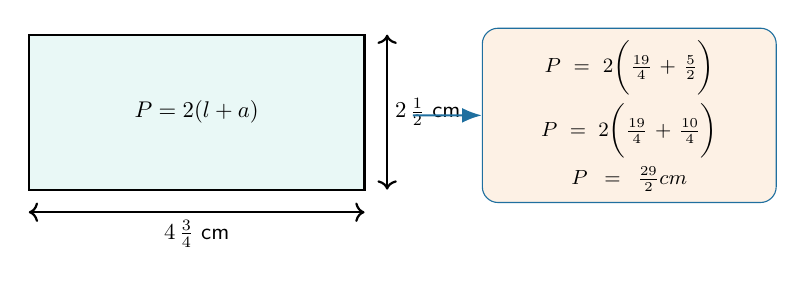
\begin{tikzpicture}[scale=0.82, transform shape]
		\draw[thick, fill=iiiepeAqua!10] (0,0) rectangle (5.2,2.4);
		\draw[thick, <->] (0,-0.35) -- (5.2,-0.35);
		\draw[thick, <->] (5.55,0) -- (5.55,2.4);
		\node[below] at (2.6,-0.35) {$4\,\frac{3}{4}$ cm};
		\node[right] at (5.55,1.2) {$2\,\frac{1}{2}$ cm};
		\node at (2.6,1.2) {$P=2(l+a)$};
		\node[cajaOp, text width=4.2cm] (perimProc) at (9.3,1.15) {
			$P=2\biggl(\frac{19}{4}+\frac{5}{2}\biggr)$\\[1mm]
			$P=2\biggl(\frac{19}{4}+\frac{10}{4}\biggr)$\\[1mm]
			$P=\frac{29}{2}\text{ cm}$
		};
		\draw[flechaProc] (5.95,1.15) -- (perimProc.west);
	\end{tikzpicture}
	\caption{Situacion 10: perimetro de un rectangulo con medidas fraccionarias.}
\end{figure}

\begin{figure}[H]
	\centering
	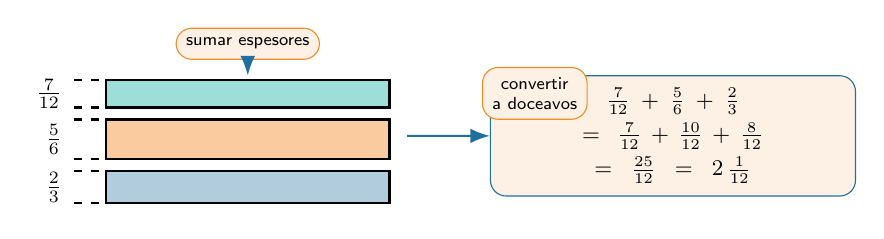
\begin{tikzpicture}[scale=0.9, transform shape]
		\foreach \y/\h/\lab/\col in {0/0.45/$\frac{2}{3}$/iiiepeBlue!35,0.62/0.56/$\frac{5}{6}$/iiiepeOrange!45,1.35/0.39/$\frac{7}{12}$/iiiepeAqua!45}{
			\draw[thick, fill=\col] (0,\y) rectangle (4,\y+\h);
			\draw[thick, dashed] (-0.45,\y) -- (0,\y);
			\draw[thick, dashed] (-0.45,\y+\h) -- (0,\y+\h);
			\node[left] at (-0.5,\y+0.5*\h) {\lab};
		}
		\node[notaProc] at (2,2.25) {sumar espesores};
		\draw[flechaProc] (2,2.02) -- (2,1.80);
		\node[cajaOp, text width=4.8cm] (tablasProc) at (8.0,0.95) {
			$\frac{7}{12}+\frac{5}{6}+\frac{2}{3}$\\[1mm]
			$=\frac{7}{12}+\frac{10}{12}+\frac{8}{12}$\\[1mm]
			$=\frac{25}{12}=2\,\frac{1}{12}$
		};
		\node[notaProc] at (6.05,1.55) {convertir\\a doceavos};
		\draw[flechaProc] (4.25,0.95) -- (tablasProc.west);
	\end{tikzpicture}
	\caption{Situacion 09: suma de espesores de tablas apiladas.}
\end{figure}

\section{Evaluacion y retroalimentacion}

\subsection{Autoevaluacion del estudiante}

\begin{table}[H]
\centering
\caption{Autoevaluacion alineada con la Sesion 02}
\label{tab:autoevaluacion-sesion02}

\small
\renewcommand{\arraystretch}{1.45}
\setlength{\tabcolsep}{5pt}
\rowcolors{2}{gray!10}{white}

\begin{tabularx}{\textwidth}{@{}
>{\raggedright\arraybackslash}X
>{\centering\arraybackslash}p{0.12\textwidth}
>{\centering\arraybackslash}p{0.14\textwidth}
>{\centering\arraybackslash}p{0.14\textwidth}
>{\centering\arraybackslash}p{0.07\textwidth}
@{}}
\toprule
\textbf{Indicador} &
\makecell{\textbf{Logrado}\\\textbf{(3)}} &
\makecell{\textbf{En proceso}\\\textbf{(2)}} &
\makecell{\textbf{No logrado}\\\textbf{(1)}} &
\textbf{Valor} \\
\midrule

Realizo sumas de fracciones de manera eficiente utilizando el algoritmo aprendido.
& $\square$ & $\square$ & $\square$ & \\

Realizo restas de fracciones utilizando de forma correcta el algoritmo.
& $\square$ & $\square$ & $\square$ & \\

Identifico correctamente la operacion para resolver un problema.
& $\square$ & $\square$ & $\square$ & \\

Justifico el denominador comun y simplifico el resultado cuando es posible.
& $\square$ & $\square$ & $\square$ & \\

Interpreto la respuesta segun el contexto del problema.
& $\square$ & $\square$ & $\square$ & \\

\bottomrule
\end{tabularx}

\end{table}

\subsection{Criterios para retroalimentar}

\begin{itemize}
	\item Si el estudiante suma denominadores, se le solicita representar las fracciones con tiras o recta numerica para recuperar que el denominador indica el tamano de la parte.
	\item Si obtiene un resultado correcto pero sin procedimiento, se pide escribir la equivalencia usada y la simplificacion final.
	\item Si confunde suma y resta en contexto, se revisa la pregunta: combinar cantidades, quitar una parte o encontrar lo que falta.
	\item Si no simplifica, se revisa el maximo comun divisor y se comprueba si numerador y denominador aun comparten factor.
\end{itemize}

% ==============================================================================
% SECCION 4: CONCLUSION
% Cierre recomendado:
% - Responder directamente a la actividad.
% - Indicar que se comprendio, no solo que se elaboro.
% - Mencionar criterio personal final.
% - No introducir informacion nueva.
% ==============================================================================
\section{Conclusion}

La actualizacion de la actividad de la Sesion 02 organiza la suma y resta con fracciones como una secuencia didactica completa: primero se recuperan conocimientos previos, despues se explica la necesidad del denominador comun, luego se practica con ejercicios graduados, se evalua mediante situaciones contextualizadas y se cierra con retroalimentacion. Esta estructura responde a los lineamientos institucionales revisados y evita que el producto se limite a una hoja de respuestas.

El criterio central es que sumar o restar fracciones significa operar partes comparables. Por eso, cada solucion debe mostrar la estrategia, el desarrollo y la verificacion. Cuando el estudiante puede explicar por que usa denominador comun, como simplifica y que significa su respuesta en el contexto, el aprendizaje deja de ser memoristico y se vuelve transferible a problemas de medida, reparto, consumo, distancia y perimetro.

% FIN DEL DOCUMENTO
\end{document}
